\documentclass{article}
\usepackage[utf8]{inputenc}
\usepackage{graphicx}
\usepackage{float}
\usepackage{subcaption}

\graphicspath{ {../images/} }

\title{Intelligent Systems - Seminar Assignment 1}
\author{Report}
\begin{document}

\maketitle

\section{Introduction}
This is a report on the 1st Seminar Assignment for Intelligent Systems class. The task was to use Genetic Algorithms to find a path out of a maze, given as an input.

The first section of the assignment was about reading the maze into an appropriate format, finding an appropriate representation of the maze and the solution, defining the fitness function (this was one of the main points here) and finding optimal settings for running the GA.

\section{Representation}
I decided to solve the problem using Python and Python library for genetic algorithms PyGAD.

I read the mazes in as NumPy arrays and represented the solutions as arrays of integers, ranging from 0 to 3. The encoding was as follows: 0 meant a move up, 1 a move down, 2 left and 3 right.

\section{Task 1}

\subsection{Fitness function}
The fitness function takes in a proposed solution and scores it. In this case it has to return a bad score if the solution goes over invalid fields (walls or out of bounds of the maze) and a good score for getting to the end of the maze, where the score for getting to the end has to be better for a solution that does not include going over walls etc. Therefore the score decreases by a constant for every invalid field and increases for every valid field, so that the GA gets a better score for moving over valid fields than simply not moving. To minimize the amount of walls that the solution crosses and maximize the probability of it finding the end, the score is strongly influenced by that. If the solution brings us to the end, the score changes by a constant, and by added parameters - it increases by the square of the number of valid points it crossed and decreases by the square of the number of invalid fields, the square of the number of times it went over the same field twice and amount of moves, to give longer paths a lower score than shorter paths. 

The biggest problem is finding a good ratio between reward and punishment - if we punish walls too much it will not make sense for the GA to go explore, since the score will be getting ever more negative with moving because of the walls. But if we increase the reward for finding the end too much, the GA will cross the walls regardless of the impact that has on the score, since the reward for finding the end is so high. That is also why the parameters like number of (in)valid fields crossed have the most impact only when finding the end.

\subsection{Other GA Parameters}
Some other the significant GA parameters:
\begin{itemize}
    \item Number of generations (iterations)
    \item Solutions per population x(population size)
    \item Number of genes (solution lengths)
    \item Crossover and mutation types and probabilities
    \item Number of parents to keep for getting the next generation
    \item Gene space and gene type - for limiting the gene values to the desired values
    \item Random seed - for replicating results
\end{itemize}

After experimenting with changing the parameters the main conclusions on their effects are the following: 
\begin{description}

\item[Number of generations] - important to allow the GA to converge, but makes execution time significantly longer with larger populations. It was set to 2000 when solving smaller mazes and to 1500 when dealing with bigger ones.

\item[Population size] - This has a big impact on performance as well. I have decided to set the population size to 100 in most cases, since it worked well with the amount of iterations.

\item[Crossover and mutation type] - Became very significant later when we wrote our own crossover and mutation functions

\subsection{Comparing results of different parameters}
As mentioned before, the size of the maze along with population size and the number of genes per solution had the biggest impact on performance, therefore those are the parameters that had to be adjusted when moving on to the bigger mazes. Switching between different crossover and mutation functions didn't have any noticeable effects on performance, but the results would vary sometimes. All-in-all the most important factor of the first task was the fitness function. 

\subsection{Results}
This basic GA with only a custom fitness function proved to be hard to fine-tune. The problem is that it is hard to determine the ratio between different penalties/rewards, no matter all the other parameters of the GA. For example, if we only decrease the score for going over invalid fields the algorithm will just loop between 2 valid fields, but if we reward the valid fields then the algorithm will still occasionally go over an invalid field. The problem complicates when we add reward for reaching the end - if the reward for reaching it is too big, then the GA won't care about not going over walls, but if it's too small, a solution that doesn't reach the end will be better because it won't get all the penalties for crossing the walls.

With that, the GA was able to solve the first three mazes semi-consistently but otherwise often insisted on passing over invalid fields, no matter the punishment. Seeing that it tends to loop, a penalty for passing a field more than once was added. Most of the score only came into the account if the end was reached, to make sure the solutions that reached it had priority over the ones that didn't. 

To avoid evaluating the GA by hand, or rather make it easier, it was compared to a solution, given by a DFS algorithm, the path plotted side by side for comparison. Despite successfully recreating the path on the smaller problems, the GA would only find significantly longer solutions on the more complex ones.
\newpage
\section{Task 2}
In the second part in the default or built-in functions for crossover and mutation were changed. I wrote and used 2 custom functions to do that

\begin{description}

    \item[Crossover function:] 
        The crossover function was improved by "educating" it about the problem, such that when doing a crossover, it would find 2 random parents and then rather than choosing a random split point, it would find the longest prefix of steps that went over valid solutions and keep that prefix and split at the next index. This way, the solutions would be directed more strongly towards the goal, since more and more solutions would keep going in the direction of valid fields. This however is only really useful in our specific problem, because if there were a lot of possible paths to take and some of those would not lead to the end, this type of crossover could get the GA stuck in a local maximum. 

    \item[Mutation function:]
        Similarly the mutation function was changed, to discourage from changing genes in a way that would bring the solution over an invalid field. The genes to be changed were, again, picked at random, but when changing a gene, the function checks if the field we reach with that gene is valid, and optionally if it means returning to the previous field. The latter is optional because sometimes it is a trade off of whether to backtrack or go over an invalid field and it will go over an invalid field, which is worse than backtracking. 
        
    \subsection{Effects of custom mutation and crossover functions}
        The custom functions helped a lot with keeping the solutions on valid paths. Running the GA with the build-in functions would often result in either a solution that got stuck in a local maxima or a solution that didn't care about passing invalid fields. The custom functions really minimized the amount of errors the GA made and provided better solutions.


	\begin{figure}[H]
		\begin{minipage}{.5\linewidth}
			\centering
			\subfloat[]{
				\label{fig:ga_default_maze3}
				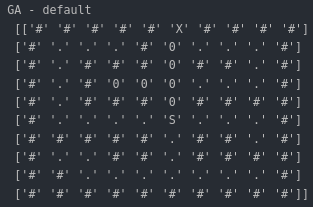
\includegraphics[scale=.4]{ga_default_maze3.png}
			}
		 \end{minipage}%
		\begin{minipage}{.5\linewidth}
			\centering
			\subfloat[]{
				\label{fig:ga_custom_maze3}
				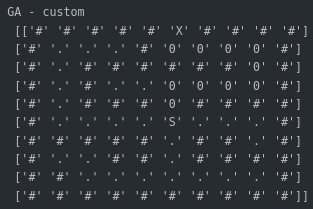
\includegraphics[scale=.4]{ga_custom_maze3.png}
			}
		 \end{minipage}\par\medskip%
		\begin{minipage}{.5\linewidth}
			\centering
			\subfloat[]{
				\label{fig:default_mutation}
				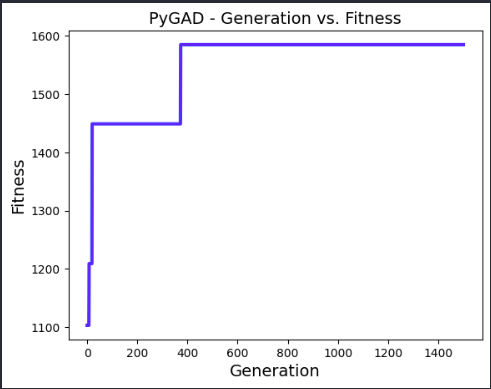
\includegraphics[scale=.25]{default_mutation.png}
			}
		 \end{minipage}%
		\begin{minipage}{.5\linewidth}
			\centering
			\subfloat[]{
				\label{fig:custom_mutation}
				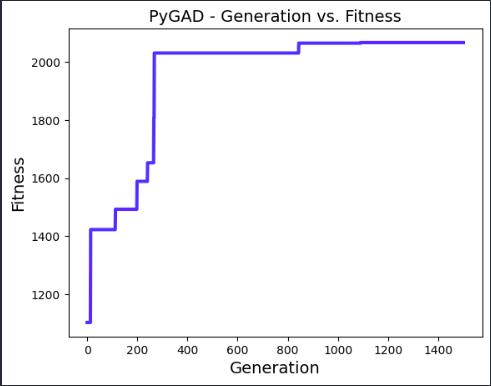
\includegraphics[scale=.25]{custom_mutation.png}
			}
		 \end{minipage}\par\medskip%
		
		\caption{
			(a)  defaults - solution; 
			(b)  custom - solution; 
			(c) default - fitness graph 
			(d)  custom - fitness graph
		}
	\end{figure}
	The pictures above depict the results of the GA with default crossover and mutation functions through the maze 3 compared to running the GA with custom crossover and mutation function. We can see that the second solution got new better solutions faster and achieved a way higher fitness score. The path on picture (a) was 100 steps long and 60 of those steps were over invalid fields, whereas the path on picture (b) was only 11 steps long and had 0 invalid moves.  This is an example of how much the custom functions helped with finding better solutions. 

The seed used for these results was 420.	
		

\end{description}        
\section{Task 3}
Task 3 introduced collection treasures hidden in the maze. My approach to this problem was to adapt the fitness function. My goal was to reward the GA for finding the treasure enough to go find it but not enough to ruin the solution. 

The first step was to add a fixed reward upon finding a treasure, but only when that treasure has not been seen yet preventing the GA from getting a high score from looping over a treasure. Since there are only a few treasures per maze the reward for finding them and the end had to be weighed extra, so if the GA found the treasures and reached the end it got rewarded by two times the number of treasures found to the power of three. Adding the reward in such way got way better results than just adding a fixed constant for finding the treasure immediately. 

This time the algorithm showed really good results and collected both treasures on 2 of the mazes, 1 on 1 and 0 on the biggest maze. This GA instance used the adapted fitness function, but the custom crossover and mutation functions as well. 

\section{Running time based on maze size}
Since this algorithm is not the most optimized - especially the parts of it that I wrote - and the length of the chromosomes grows with the number of fields in a maze, the execution time gets relatively long with bigger mazes.

\begin{figure}[H]
	\begin{minipage}{.9\linewidth}
		\centering
		\subfloat[] {
		\label{fig:execution_times}
		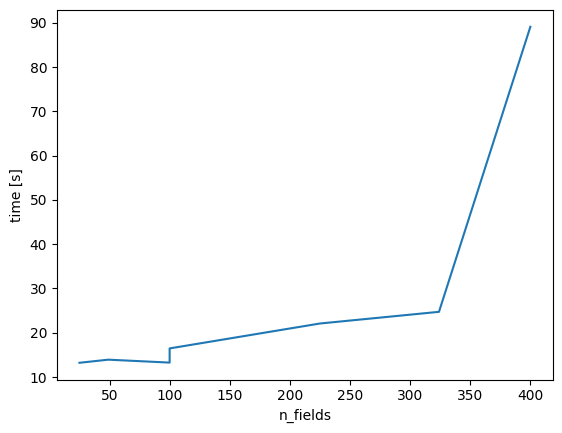
\includegraphics[scale=.5]{execution_times.png}
	}
	\end{minipage}%
	\caption{Bar chart of running time per number of fields in a maze}
\end{figure}

As can be depicted from the chart above, the execution time grows very fast with the number of fields in the maze, given that all the other parameters stay the same.

\section{Conclusion}
The GA resulting from this assignment still has a lot of room for improvement, but a significant portion of improvements lies in fine-tuning the parameters. The results might also be drastically different if I had the resources to run the GA for many more iterations, but that would take too long to test. The given task is also not well suited to genetic algorithms.

The algorithm will sometimes still choose invalid solutions, which means the fitness function needs improving, however at the time I have not come up with a better solution. Having tried many parameter combinations this is the best I got to, even though one combination of settings might work better on one maze and worse on another. 

\end{description}
\end{document}
